\chapter{Function calls with timeouts}
\label{chap:functions}

\ifdefined\chapquotes
\begin{chapquote}{Isaac Asimov, \textit{The Gods Themselves}}
`Does everyone just believe what he wants to?' \\
`As long as possible.  Sometimes longer.'
\end{chapquote}
\fi

In this chapter, we introduce the design of lightweight preemptible functions, our
abstraction for making ordinary function calls with a timeout.  We will cover the
implementation in Chapter~\ref{chap:libinger}, after the intervening chapters have
introduced a supporting abstraction for memory isolation and shown how to use it.

One thing that distinguishes preemptible functions is that their invocation is
synchronous;
that is, the program does not continue executing the code following the call until
the callee has made some progress (though not necessarily run to completion).  This
stands in contrast to abstractions with asynchronous invocation.  The thread and
callback-based future abstractions are like preemptible functions in that structuring
code for them involves writing a function describing the task (a thread main function
or a callback, respectively).  But these traditional abstractions differ in that this
function does not necessarily
begin executing until later:\@ a scheduler or event loop in the runtime or operating
system manages all of the program's tasks and decides when to invoke each one.

The other distinguishing feature of preemptible functions is that they are
preemptive, meaning that interruption is external and can occur at (almost) any point
in their execution.  Abstractions such as futures and user threads are generally
cooperative.  As such, interruption is internal and control transfers to another task
only when the executing one explicitly yields control (or calls a library function
that does so on its behalf).  Table~\ref{tab:invokeinterrupt} classifies concurrency
abstractions based on their type of invocation and interruption.

\begin{table}
\begin{center}
\begin{tabular}{r r | c c}
&& \multicolumn{2}{c}{task interruption} \\
&& cooperative & preemptive \\
\hline
& \\
\multirow{3}{*}{\rotatebox{90}{task invocation}} & \multirow{2}{*}{asynchronous} & user threads & \multirow{2}{*}{kernel threads} \\
&& callback-based futures \\
& \\
& synchronous & ``async'' futures & \textbf{preemptible functions} \\
&& (\texttt{async}/\texttt{await}) \\
& \\
\end{tabular}
\end{center}
\caption{Concurrency abstractions classified by type of invocation and interruption}
\label{tab:invokeinterrupt}
\end{table}

From the table, it is apparent that the term \textbf{asynchronous} is overloaded.
In the context of invocation, it is synonymous with ``background.''  Confusingly, in
the context of futures, async functions are those that can use the \texttt{await}
keyword to insert a yield point that takes a \textit{synchronous} function call off
the critical path.  POSIX has a third meaning for the term:  In the context of
signals and cancellation, it means ``preemptive.''  Examples of this usage include
the phrases ``asynchronous cancellation'' and ``async safety.''


\section{Motivation}
\label{sec:functions:motivation}

\begin{figure}
\begin{center}
\includegraphics[width=0.65\columnwidth]{functions/figs/progsupport}
\end{center}
\caption[Taxonomy of support for library code]{
Taxonomy of support for library code.  It is difficult to determine whether
a library is fully reentrant, so in practice we always
apply one of the two mitigations.  Library copying is used by default, but deferred
preemption is needed to preserve the semantics of \texttt{malloc()} and users of
uncopyable resources such as file descriptors or network adapters.}
\label{fig:progsupport}
\end{figure}

\begin{swallowsections}
\begin{swallowfigures}
\input[functions]{intro}
\end{swallowfigures}
\end{swallowsections}


\input[functions]{related}

Some recent languages offer explicit userland threading, which can be used to
support timed code.  One example is the Go language's~\cite{www-golang}
\textit{goroutines}, which originally relied on a cooperative scheduler that
conditionally yielded at function call sites.  This caused real-world problems for
tight loops, requiring affected programmers to manually add calls to the
\texttt{runtime.Gosched()} yield function~\cite{www-golang-tightloop}.  To address
this, the language eventually migrated to a preemptive goroutine
scheduler~\cite{www-golang-rel14notes}.

\input[functions]{related_gofigure}


\section{Preemptible functions: \textit{libinger}}

We observe that today's concurrency abstractions offer either synchronous invocation
or preemptive scheduling, but not both.  On one hand we have futures, which are now
synchronous\footnote{Code interfacing with futures via the ``async/await''
continuation passing style is now prolific.} but purely cooperative.  On the other
are kernel threads, which are preemptive but asynchronous.  We bridge this gap by
introducing a novel abstraction that provides synchrony \textit{and} preemption for
unmanaged languages.

Doing so requires confronting the very nonreentrancy problems that have long doomed
attempts to support asynchronous cancellation outside of purely functional contexts.
This turns out to be a slightly harder problem than safely supporting concurrency, so
in addition to cancellation, we get the ability to externally pause for free.

\begin{swallowsections}
\input[functions]{inger_inger}
\end{swallowsections}


\subsection{Design principles}

Although we are introducing a new concurrency abstraction, we have striven to keep
the interface simple and understandable.  The following design principles have guided
this effort:
\begin{itemize}
\item \textbf{We do not assume that users need asynchrony.}  Hence, preemptible
	functions \textit{run on the same kernel thread as their caller}.  This is
	good for performance (especially invocation latency), but it is also
	important to be aware of; for instance, it means that a preemptible function
	will deadlock if it attempts to acquire a lock held by its caller, or vice
	versa.  Of course, some users may need asynchrony.  The preemptible function
	abstraction composes naturally with both threads and futures
	(Chapter~\ref{chap:libturquoise}), so there is no need to reinvent the wheel.
\item \textbf{We assume that simply calling a preemptible function is the common use
	case.}  As such, the \texttt{launch()} wrapper both constructs and invokes
	the preemptible function rather than asking the user to first employ a
	separate constructor.  Users wishing to separate the construction and
	invocation operations can pass the sentinel \texttt{0} as the
	timeout, then later use \texttt{resume()} to start execution.
\item \textbf{We favor a simple, language-agnostic interface.}  The fact that our
	interface centers on a higher-order function in the style of the
	\texttt{pthread\_create()} and \texttt{spawn()} wrapper functions means that
	using preemptible functions looks similar regardless of the programming
	language.  Currently, \textit{libinger} provides bindings for both C and
	Rust.  If and when we add bindings for other languages, we expect them to
	have the same feel; in the meantime, other languages can use preemptible
	functions (unsafely) through their C
	foreign-function interfaces.  We considered adhering to the futures interface
	instead, but decided against it because each language has its own
	incompatible variant thereof.  The relative ease of building a futures
	adapter type (Chapter~\ref{chap:libturquoise}) affirms our decision.
\item \textbf{We keep argument and return value passing simple yet extensible.}
	Because Rust supports closures, the Rust version of \texttt{launch()} accepts
	only nullary functions:\@ those seeking to pass arguments should just capture
	them from the environment.  C supports neither closures nor generics, so the
	C version of \texttt{launch()} accepts a single \texttt{void *} argument that
	can serve as an in/out parameter.  It occupies the last position in the
	parameter list to permit (possible) eventual support for variable argument
	lists.
\item \textbf{We choose defaults to favor flexibility and performance.}  When a
	preemptible function times out, \textit{libinger} assumes the caller might
	later want to resume it from where it left off.  As such, both
	\texttt{launch()} and \texttt{resume()} pause in this situation; this incurs
	some memory and time overhead to provide a separate execution stack and
	package the continuation object, but exhibits lower latency than
	asynchronous cancellation.  If the program does require cancellation, we
	provide ways to explicitly request it (Chapter~\ref{chap:libinger}).
\item \textbf{In addition to preemption, we offer the option to yield.} This feature
	enables the construction of higher-level synchronization constructs tailored
	to preemptible functions (Chapter~\ref{chap:libinger}).  It also allows
	preemptible functions to coexist with cooperatively-scheduled tasks
	such as futures (Chapter~\ref{chap:libturquoise}).
\end{itemize}


\section{The preemptible functions ecosystem}
\label{sec:libinger:concurrency}

In divorcing preemption from asynchronous invocation, preemptible functions
disentangle interruption from parallelism.  Indeed, \textit{libinger} does not
provide a task scheduler because the only decision it makes is whether to pause the
currently executing code.  Whenever it opts to do so, it unconditionally returns
control to the preemptible function's caller.

This design allows client code to pick and choose the level of runtime support it
needs.  If it only invokes preemptible functions synchronously and makes all
scheduling decisions itself, it can link directly against \textit{libinger} and use
the interface presented in Section~\ref{sec:libinger}.  If it prefers to delegate
scheduling to a runtime, we also provide \textit{libturquoise}, a preemptive futures
executor offering an event loop and thread pool
(Chapter~\ref{chap:libturquoise}).

Figure~\ref{fig:architecture} shows the dependency relationship between
\textit{libinger} and \textit{libturquoise}, in the context of the other software
components developed for this thesis.  Notably, both libraries support nonreentrancy
by depending on another library called \textit{libgotcha}, which provides a novel
abstraction of its own for enforcing isolation boundaries.  The \textit{libinger}
library is implemented in approximately 2,500 lines of Rust; \textit{libgotcha}
comprises another 3,000 lines of C, Rust, and x86-64 assembly.

\begin{figure}
\begin{center}
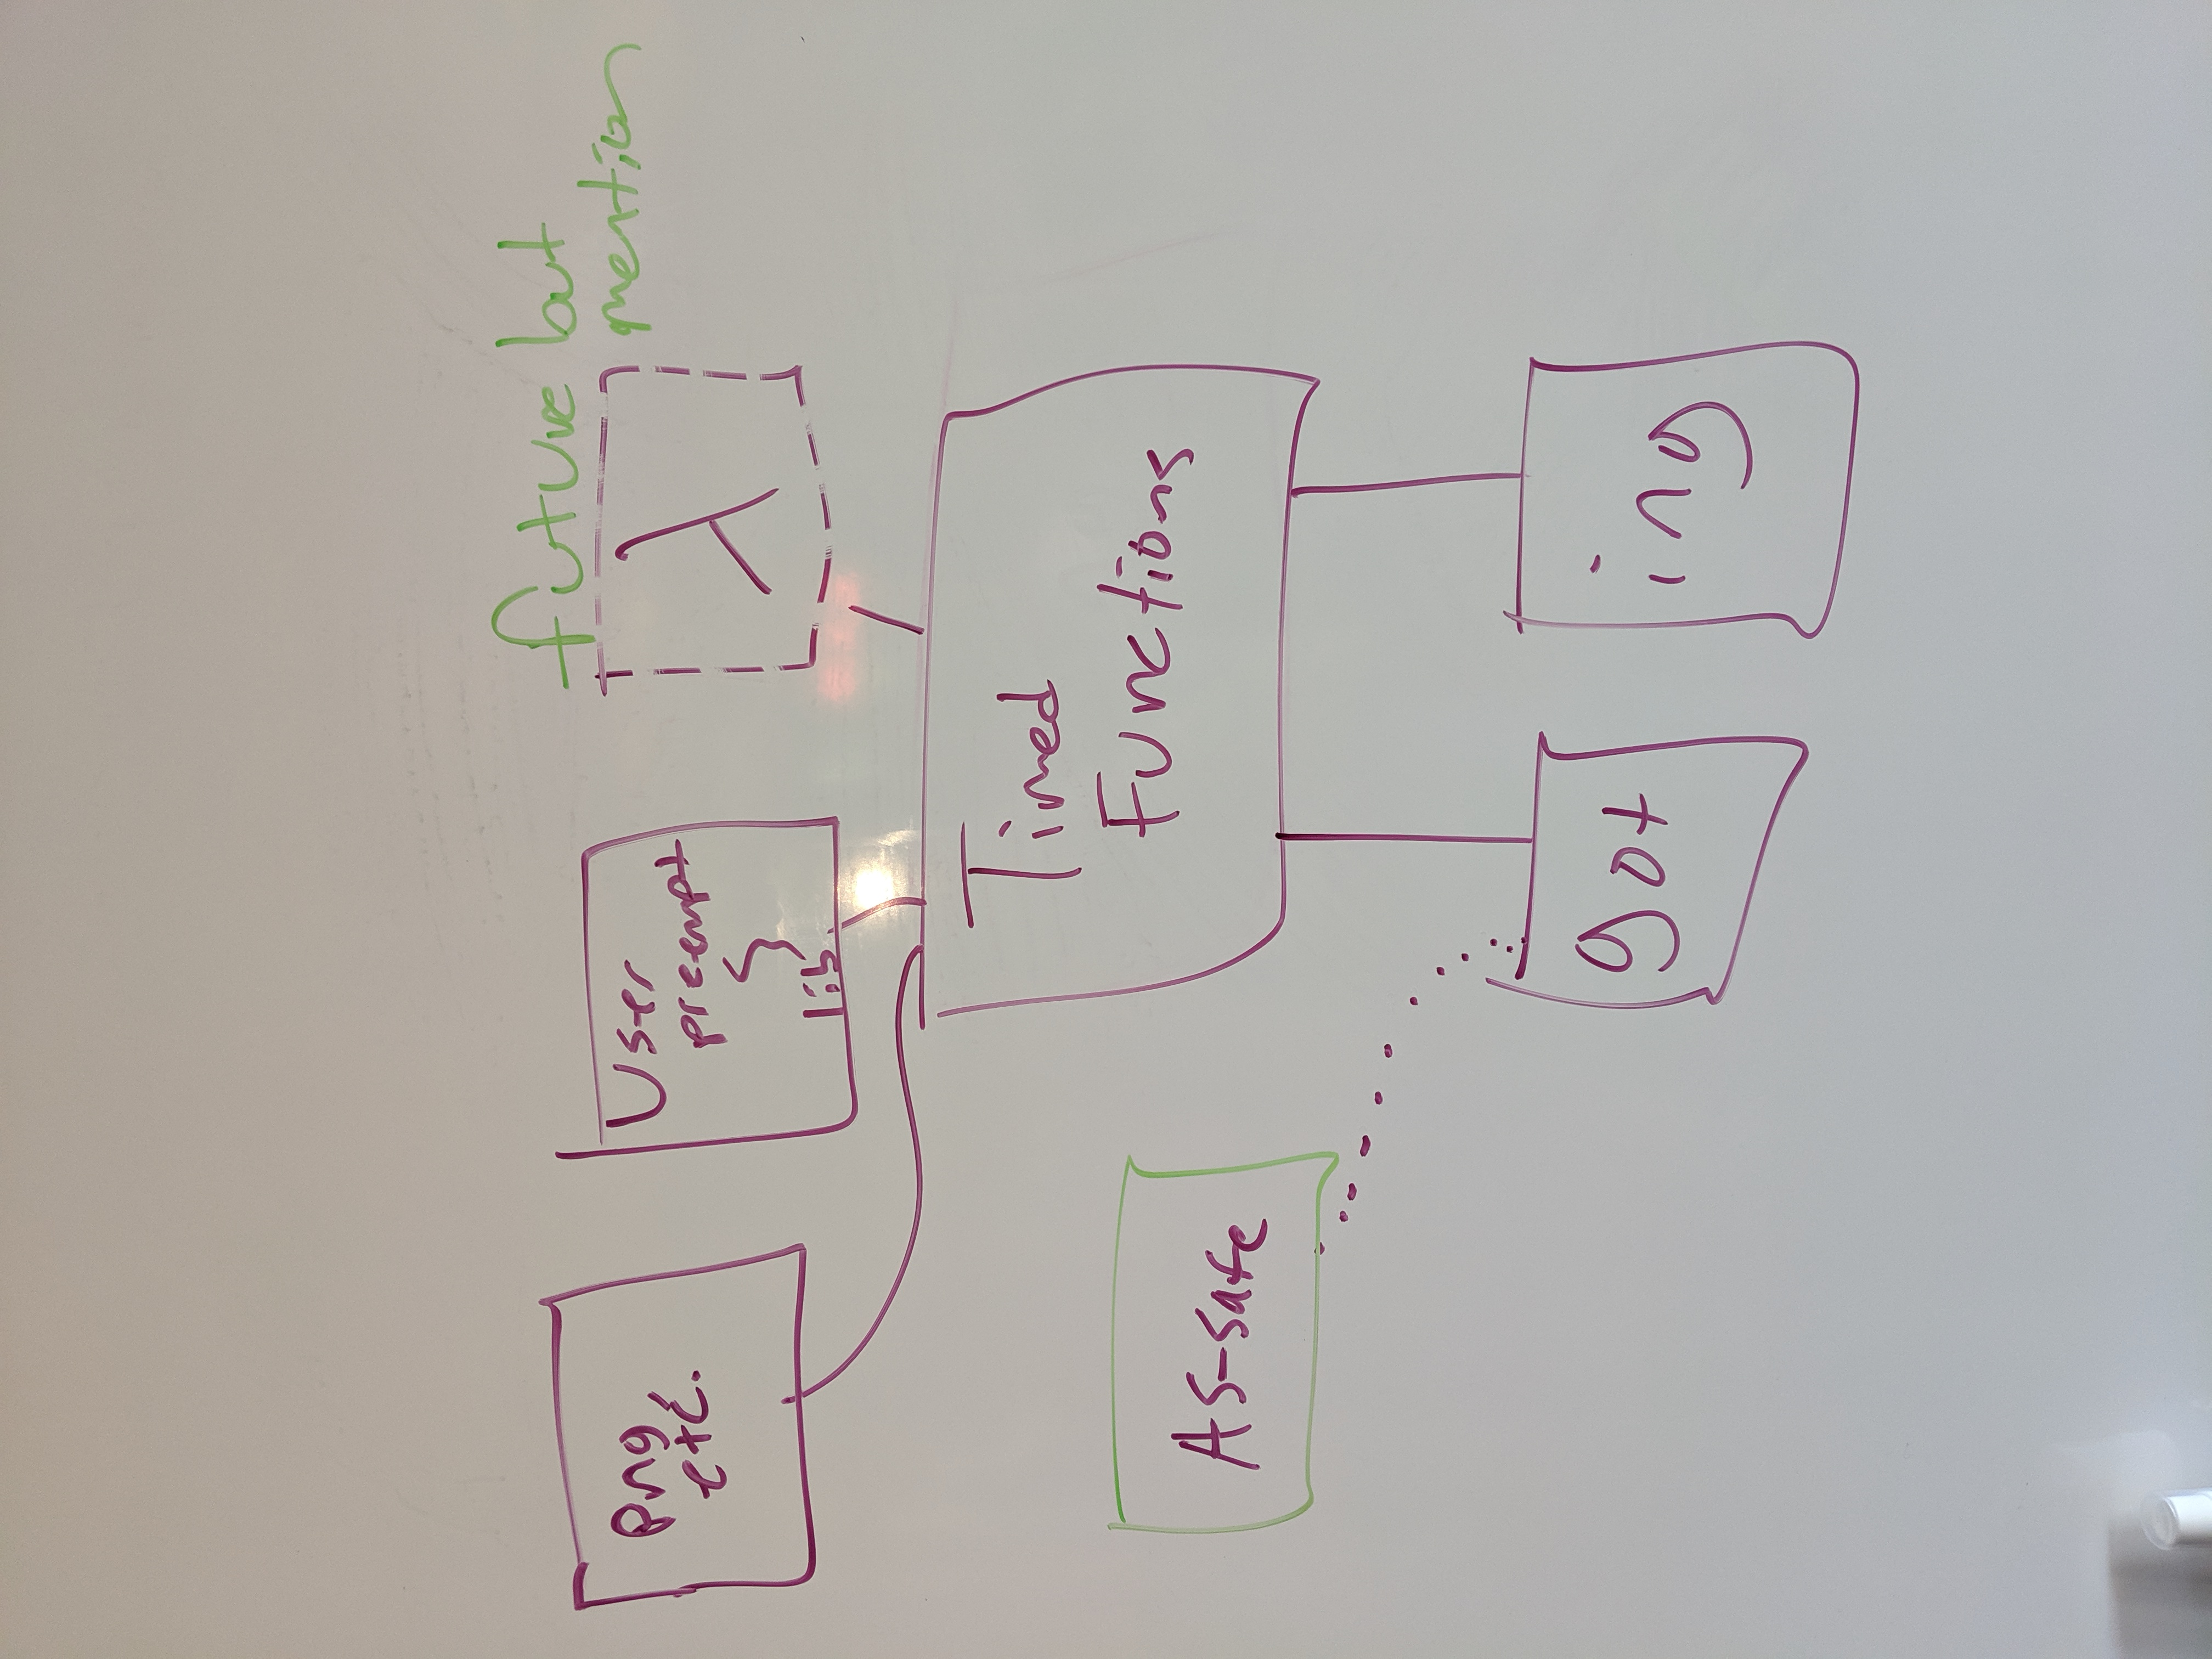
\includegraphics[width=\columnwidth]{functions/figs/architecture}
\end{center}
\caption[Preemptible functions software stack]{
Preemptible functions software stack.  Hexagonal boxes show
the required runtime environment.  Rectangular boxes represent components
implementing the preemptible functions abstraction.  Ovals represent components built
on top of these.  A preemptible function's body (i.e., \texttt{func}) may be defined
directly in
your program, or in some other loaded library.}
\label{fig:architecture}
\end{figure}


\subsection{Automatic handling of shared state: \textit{libgotcha}}

\begin{swallowsubsections}
\input[functions]{inger_gotcha}
\end{swallowsubsections}

Note that preemptible functions are still a concurrency abstraction, and our
automatic handling of shared state internal to dependencies does not exempt the
author of a preemptible function from writing safe concurrent code.
